\documentclass[]{article}
\usepackage{amssymb}
\usepackage{amsmath}
\usepackage{amsthm}
\usepackage{graphicx}
\usepackage{hyperref}


\newtheorem{theorem}{Theorem}
\newtheorem{conjecture}[theorem]{Conjecture}
\newtheorem{corrollary}[theorem]{Corollary}
\newtheorem{lemma}[theorem]{Lemma}
\newtheorem{example}[theorem]{Example}


\DeclareMathOperator*{\argmax}{\text{argmax}}
\DeclareMathOperator*{\argmin}{\text{argmin}}
\DeclareMathOperator{\uu}{\mathbf{u}}
\usepackage{tikz}
\usetikzlibrary{calc, shapes, fit}

% Title Page
\title{Spatially Structured Coordination Games and their Applications in Theoretical Ecology}
\author{John McAlister}



\begin{document}
\maketitle

\begin{abstract}
	In the well understood $2\times 2$ coordination game, players are incentivized to take on the same strategy as their opponents. When the coordination game is played over a network of many individuals, the dynamics are much more complicated and, when no strategy is inherently better than another, we see many non-trivial equilibria.  The question of how pairwise interactions and networks of association can lead to coordination behavior is of interest to economists and ecologists alike. With this project we seek to understand the equilibria of coordination games, played on domains with spatial structure, in more generality. First, we will investigate the qualities of the equilibria of this game in discrete space and their stability. Next, we will attempt to build an algorithm which can find equilibrium solution in discretely structured space given a set of boundary values. Finally, we will extend our investigation to continuous space to think about how the interaction between familiarity and strategic recognition can determine when strategic gradients can exist in space. We believe that each of these questions provides us with a new and unique way of considering coordination behavior in space. 
\end{abstract}
	\section{Introduction}\label{introduction}
	\subsection{Economic Background}\label{economicbackground}
		The Coordination game, at its most basic, is a two player game with the following payoff matrix
		With the assumption that $a>d$ and $b>c$.
		\begin{figure}[h!]\label{twobytwopayoff}
		\begin{center} 
			\begin{tabular}{c|cc}
				&A&B\\
				\hline 
				A&a,a&c,d\\
				B&d,c&b,b
			\end{tabular}
		\end{center}
		\caption{The Payoff matrix for the $2\times 2$ coordination game}
		\end{figure}
		It has two pure strategy Nash equilibria, $(A,A), (B,B)$, and a mixed strategy Nash equilibrium where both players play strategy $A$ with probability $p=\frac{b-d}{a+b-c-d}$. On its own, the two player game with two strategies is entirely understood\cite{Maschler2013}. 
		The game can also be considered among many players where pairs of players are selected to play uniformly randomly. During the rise in popularity of evolutionary game theory in the 1990s, economists began to consider the game as a way of answering the question: how do communities decide between behaviors when it is beneficial to use the same strategy. The canonical example is many people in an office choosing operating systems. Those who are using the same operating system will have an easier time working together than those who use different operating systems, but neither operating system provides more utility over the other individually. 
		
		Among the first to consider this game were Kandori, Michihiro and Rob, who investigated a system with high inertia and $\varepsilon$-noise. In their system, they imagined all players were paired up uniformly to play the coordination game. Occasionally a player is able to update their strategy by myopic best response. Additionally, rare mutations occur where a player's strategy changes uniform randomly. In their investigation, they found that when the system is allowed to proceed as described, it will converge to the risk dominant Nash equilibrium\cite{Kandori1993}. Another study by Robson and Vega-Redondo showed that which equilibrium is selected for is sensitive to the way in which players were paired up. They described a match selection procedure that would select for the Pareto dominant Nash equilibrium, even when it did not coincide with the risk dominant Nash equilibrium\cite{Robson1995}. 
		
		In either case described above and in other similar studies \cite{Kandori1995}, all players are assumed to interact with one another with equal probability. However, in the system at hand, this assumption is unreasonable because, as networks grow, individuals cannot interact with everyone else in the network. Moreover, it was shown by Ellison that the convergence in these systems was unreasonably slow to sufficiently describe coordination behavior in the economic setting \cite{Ellison2000}.
		
		Newer models addressing these concerns started looking at non-uniform player selection. The most natural way to think of this is as a graph in which players are vertices which share edges when there is a non-zero chance they will be paired up. Adding this spacial structure complicates the game significantly. The previous models can be thought of as a structured game played on complete graphs; when the graph in incomplete, the dynamics of the game are more complicated. 
		
		Ellison was the first to attempt this kind of model in the economics literature. He suggested that players were constantly updating (unlike the high-inertia assumption from previous models) and that there was still some $\varepsilon$-noise. Additionally, not all players were paired up with one another, rather players were arranged in a circle and would associate only with the vertices close to them in the circular arrangement\cite{Ellison1993}. This configuration, which has come to be called the ``circular city" \cite{Weidenholzer} still has a great deal of symmetry, which reduces the state space considerably. In addition to the circular cities, Ellison investigated square lattice configurations. In each case he showed similar results about convergence to the risk dominant equilibrium, although in the low inertia case, the convergence is, unsurprisingly, much faster. 
		
		Each of these previous studies have taken the approach of using symmetry to reduce the state space, considering a transition matrix without noise and establishing a distance between states through mutation. Without a way to reduce the state space in general, this approach becomes intractable for general graphs. Moreover, the fact that there are only two available strategies in many of these early models and the fact that there is constant noise means that unstable equilibria, or equilibria with many different strategies present, have been entirely overlooked. 

		\subsection{The Model}\label{themodel}
		In the model proposed here, we seek to consider a general graph with no noise in order to understand the properties of equilibrium strategy profiles and produce separate stability criteria, rather than simply seeking out the trivially stable trivial equilibrium. 
		
		Consider this most general setting: For a connected graph $G(V,E)$ each vertex $v\in V$ plays a strategy $c$ from a set of pure strategies $C$, and the payoff for $v$ is given by \begin{equation}\label{fitness1}
			w(v,c|\uu)=|\{x\in \Gamma (v);\uu_x=c\}|
		\end{equation}
		where $\uu$ is the strategy profile, $\uu_x$ is the strategy that vertex $x$ is using, and $\Gamma(x)$ is the set of vertices which share an edge with $x$. 
		In this case, the game is at its most simple where the Payoff matrix is simply $I_n$. Note, however, we are not limited to only two strategies as before. 

		In keeping with the previous work, we use a myopic best response as our replicator dynamic. In this way we construct a sequence of strategy profiles $\uu(t)$ with 
		\begin{equation}\label{dsys}
			\uu_v(t+1)\in \argmax_{c\in C}\{w(v,c|\uu(t))\}.
		\end{equation}
		It may be that $|\argmax|>1$, so we break ties in the following way, which could be describes as $\varepsilon$-inertia. If $\uu_v(t)\in \argmax_{c\in C}\{w(v,c|\uu(t))\}$, then $ \uu_v(t+1)=\uu_v(t)$. If not, $\uu_x(t+1)$ is selected from $\argmax_{c\in C}\{w(v,c|\uu(t))\}$ uniform randomly. This is unlike the high inertia assumption from the economists; we only assume that changing strategy comes with some ``menu cost," which is less than any non-zero benefit a vertex could receive by switching strategies.  
		\subsection{Areas of Investigation}\label{areasofinvestigation}
		Here we have described a evolutionary game which can be imagined as discrete time, discrete state dynamical system. It is clear to see that Equilibria in the dynamical system are Nash Equilibria of the game. There are many potentially interesting questions that arise from this system.
		
		First, in section \ref{equilibria and stability},  we seek to Characterize Equilibria for a general graph and determine stability conditions. If we assume that an equilibrium exists, we seek to understand necessary conditions about these equilibrium strategy profiles through methods in extremal graph theory, and to determine their stability through typical linear algebraic methods. 
		Next, in section \ref{boundaryvalueproblem}, we will consider what a ``boundary value problem" of this sort may look like. Given a set of boundary conditions, we hope to find a strategic interpolation that is a Nash Equilibrium. To do this, we intend to use techniques from graph partitioning and community detection. 
		Lastly, in section \ref{continuousvariations}, We consider some strategically continuous variations of this game and use them to investigate evolution of cooperative behavior. Together, these investigations are unified by a common theme of spatially structured coordination with the goal of going beyond previous economic results to a more general class of spatial structures.
		
	
	
	\section{Equilibria and Stability}\label{equilibria and stability}
	\subsection{Describing Equilibria}\label{describingequilibria}
	\begin{figure}
		\includegraphics[width=0.4\linewidth]{images/OralFig2v3}
		\includegraphics[width= 0.4\linewidth]{images/OralFig3v4}
		\caption{\textbf{Left} A trivial equilibrium in a 4-regular graph. \textbf{Right} a non-trivial equilibrium with $3$ clusters in a 4-regular graph. In both, the strategies used by each vertex are represented by the color of the vertex.}
		\label{equilibria}
	\end{figure}
		
		The dynamical system \eqref{dsys}, and its corresponding evolutionary game, clearly have a trivial equilibrium (Fig. \ref{equilibria} Left). Indeed, in every graph, the strategy profile $\uu_x=c$ for all $x\in V$ is an equilibrium. We call this the Trivial equilibrium. The proof that it is an equilibrium is direct from the definition of Nash equilibrium so it is not worth discussing further. Of more interest to us are the plentiful non-trivial equilibria which are admitted by most (but not all) graphs (Fig \ref{equilibria} Right). In this section, it will be our goal to characterize the non-trivial equilibrium strategy profiles for general graphs.  
		
		In order to discuss these ideas we need a definition. We say a cluster is a subgraph of $G$ spanned by all of the vertices using a particular strategy. We will use the following notation.  We write $Q(\mathbf{u})$ to mean the set of all clusters in a strategy profile $\mathbf{u}$. We write $q^c$ to mean the cluster in $Q(\mathbf{u})$ in which vertices use strategy $c$. Lastly, we write $\partial q^c$ to mean the set of vertices in $q_c$ which have neighbors in other clusters.

		Unsurprisingly, it is not an easy task to produce a set of conditions on equilibrium strategy profiles for a general graph, so the first step is to consider equilibria of special graphs with nice properties. Below are two theorems about equilibria for special classes of graph for which we can classify all the admitted equilibria.
		\subsection{Simple Graphs with Nice Properties}\label{simplegraphswithniceproperties}
		\begin{theorem}\label{KnTheorem}The only equilibrium in $K_n$ is the trivial equilibrium.
		\end{theorem}
		\begin{proof} 
			Suppose by way of contradiction there is an equilibrium strategy profile $\mathbf{u^*}$ with $d\geq2$ clusters, $q^{c_1},...,q^{c_d}$. Because every pair of vertices shares an edge,
			\begin{equation}\label{Knfitness}
				w(v,c_i|\uu)=\begin{cases}
					|q^{c_i}|&\uu_v=c_i\\
					|q^{c_i}|-1&\uu_v\neq c_i
				\end{cases}
			\end{equation} so the fitness of a vertex is directly associated with the size of the cluster of which it is a part.  Consider a vertex $v_1\in q^{c_1}$. Because it is at equilibrium, $$w(v_1,c_1|\uu^*)=\max_C\{w(v_1,c|\uu^*)\}=:a.$$
			Therefore, $|q^{c_1}|=a+1$. Moreover, the fitness of $v_1$ if it played a different strategy $c_2$ would be  $w(v_1,c_2|\uu^*)\leq a$ so $|q^{c_2}|\leq a$.
			Now consider a separate vertex, $v_2\in q^{c_2}$. $w(v_2,c_2|\uu^*)=|q^{c_2}|-1\leq a-1$ by  equation \eqref{Knfitness}. However, $w(v_2,c_1|\uu^*)=a+1$. 
			Thus $\uu^*_{v_2}=c_2\notin \argmax\{w(v_2,c|\uu^*)\}$, so $\uu^*$ is not an equilibrium.  
		\end{proof}

		Although this theorem does not comment on the flow of a system from an initial condition to the trivial equilibrium, it is consistent with the findings of the economists in the unstructured setting. When all strategies offer equal fitness and there is no risk dominant equilibrium, then the system, if it converges, must converge to the trivial equilibrium. In this system, however, it is not necessarily true that the system converges to an equilibrium, it may also converge to a 2-cycle which will be discussed later in the section. 
		
		\begin{theorem}\label{KnnTheorem}{$K_{n,m}$ admits an equilibrium with $d$ clusters if and only if $d|n$ and $d|m$.}
		\end{theorem}
	
		\begin{proof} Consider the complete bipartite graph $K_{n,m}$ which has parts $E^n$ and $E^m$, with $n$ and $m$ vertices, respectively. 
			
			 
			$\impliedby$ Let $d$ be a common divisor of $m$ and $n$. It is sufficient to construct an equilibrium strategy profile with $d$ clusters. Partition the vertices of $E^m$ so that there are $m/d$ vertices using each strategy. Likewise, partition the vertices of $E^n$ so that there are $n/d$ vertices using each strategy. Consider $v_1\in E^m$.  Notice, because it shares an edge with every vertex in $E^n$ its fitness is certainly 
			\begin{equation}
				w(v_1,c|\uu)=\frac{n}{d}\quad \forall\, c\in C
			\end{equation}
			Therefore, it is certainly playing a best response. The same can be said for every vertex in $E^n$. Thus we have constructed an equilibrium with $d$ clusters.
			
			
			$\implies$ I argue by contradiction.   Without loss of generality, suppose that $d$ is not a divisor of $m$. Suppose $\uu^*$ is an equilibrium strategy profile with $d$ clusters. $d$ does not divide $m$, so $\exists$ strategies $r$ and $s$ such that $|q^r\cap E^m|>|q^s\cap E^m|$. If $\uu^*$ is at equilibrium, it must follow that $q^s\cap E^n=\emptyset$. It then follows $q^s\cap E^m =\emptyset$. If $q^s$ is empty then there are not $d$ clusters in $\uu^*$. This contradiction proves that if there is an equilibrium strategy profile in $K_{n,m}$, the number of clusters must be a common divisor of $n$ and $m$.   
		\end{proof}

		\subsection{More General Approaches}\label{moregeneralapproaches}
		For special graphs like the ones discussed above, classifying all the equilibria can be simple; for general graphs the problem is not as simple. In general, the process of finding equilibria is equivalent to finding a vertex partition with the following condition:
		\begin{equation}
			\mathcal{P}= \left\{P^{c}\right\}_{c\in C}\text{ where } x\in P^{c}\Rightarrow |\Gamma(x)\cap P^{c}|\geq |\Gamma(x)\cap P^{c'}|\, \forall c'\in C. 
		\end{equation}
		There are other similar kinds of graph partitions, like the modularity partition or the minimum cut partition, which will be discussed heavily in section \ref{boundaryvalueproblem}. 
		Problems in community detection rely heavily on these partitions but the game theory and economics literature has not relied on insights from this field. Despite the similarities, this disconnect is natural when we pose the questions as an initial value problem. Without more restrictions on the partition we run into problems. For instance, we do not know a priori how many strategies will be present in an equilibrium (equivalently, how many parts the graph will be partitioned into)\cite{Newman2006}. Moreover, it is not assumed that a non-trivial equilibrium (non-trivial partition) exists, so partitioning algorithms are not guaranteed to be useful.
		Additionally, sub-optimal equilibria are still of interest to us, but may be missed by partitioning algorithms\cite{Clauset2004}.  All this is to say that, when we consider this system as an initial value problem, the insights offered by typical graph partitioning can only take us so far. 
	
		To support what can be learned from the partitioning approach in this context we also want to investigate equilibria through other means. Energy-like estimates are one method,
		%Is a citation necessary?%
		inspired by differential equations, which could help us to describe flows and basins of stability. The barrier to this so far is the absence of a suitable energy. Neither $1-Q$ (modularity) nor the number of edges which connect different clusters are appropriate energies for this context. Although both describe the community structure of a strategy profile (and indeed are used in graph partitioning) we do not get useful results (like monotonicity) from either energy. 
		
		While finding an appropriate energy measurement will help describe flows in the system, results from extremal graph theory will help us predict possible equilibria from the graph structure in which it may exist. The goal will be to describe necessary conditions on cluster boundaries using the fact that these boundaries contain a vertex set which is like a separating set\cite{ExtremalGraphTheory}. One goal, which may fall into this area but is discussed later in section \ref{boundaryvalueproblem}, is the determination of the number of cluster that may be admitted by a graph just by the properties of the graph itself. 
		\subsection{Numerical Results}\label{numericalresults}
		To support these methods, we may also rely on numerical findings. Despite the complexity of predicting equilibria from a graph and understanding its basins of stability, the dynamical system itself is quite straight forward to simulate and thus numerical findings are readily available to support our analytical goals. 
		
		For instance, there is an intuitive relationship between the edge density of a graph and the number of clusters it may admit at equilibrium. We can explore this relationship by generating many random graphs and finding equilibria by giving random initial conditions and solving the initial value problem (Fig. \ref{NumericalScan}). 
		\begin{figure}
			\includegraphics[width=\linewidth]{images/KregNumericalScan}
			\includegraphics[width = \linewidth]{images/WSNumericalScan}
			\caption{A scatter plot showing the cluster number and edge density of many limits (equilibria or 2-cycles) in randomly generated $k$-regular graphs (above) or Watts-Strogatz graphs (below) given random initial conditions.}
			\label{NumericalScan}
		\end{figure}
		
		%%Section here Showing off how good the numerics are
		
		It is crucial to point out that when viewed like an initial value problem, it is not always true that a sequence of strategy profiles converge to an equilibrium. It is very common for cycling to occur (Fig. \ref{cycle}). We see that these are quite common when we simulate these systems. However, it is interesting to note that $n$-cycles with $n\geq 3$ have never been observed. Indeed, we conjecture that such a cycle is, in general, impossible although we do not yet have a proof. Any $n$-cycle is a result of the simultaneous update that governs the behavior of the system. If the same game were to be played with sequential update (equivalent to the high-inertia setting described in the Introduction), then no such cycling can exist because every update can only reduce the number of edges which connect vertices of different strategies. (That is to say, the number of edges connected different clusters is an appropriate energy in the sequential case).
		
		\begin{figure}
			\includegraphics[width =  \linewidth]{images/OralFig4v2}
			\caption{Two strategy profiles which together make up a 2-cycle. In the profile on the left, every vertex is playing its best response to the profile on the right and the same is true the other way around.}
			\label{cycle} 
		\end{figure}
		\subsection{Stability}\label{stability}
		In addition to understanding equilibria structurally, we also aim to classify equilibria by their stability. The first and most approachable way we will think of stability is as local stability. We say a vertex is locally stable if the perturbation of a single nearby vertex will not change the strategy of the original vertex in the next iteration. This is equivalent to the vertex being at a \textit{proper} fitness maximum (the $\argmax$ is of size 1). 
		
		The natural next stability concept is global stability where every vertex is locally stable. We seek to find a more easily checkable algebraic condition than confirming that every vertex is at a proper fitness maximum. The global stability concept is definitionally identical to the Evolutionary Stable Strategy concept from evolutionary game theory\cite{Apaloo2009,Nowak2006} but to properly discuss flows in this dynamical system we need a stronger concept like convergent stability. The idea that ``near by" strategies will converge to a given equilibrium with probability 1 requires a definition of ``near by" which is less clear in the discrete case when strategies do not exist in a vector space. However, strategy profiles can be compared using the metric $d(\uu_1,\uu_2)=\sum_{v\in V}(\delta(\uu_{1,v},\uu_{2,v}))$.
		
		In a similar way, it may be interesting to discuss invaisability of certain equilibria. Returning to the original inspiration for this project, understanding when novel cooperative behaviors can invade or when equilibrium strategy profiles resist invasion, can give insights into the evolution of cooperative behaviors.
		
		The final stability concept we offer is the structural stability concept. This concept is very unlike the previous four because it has to do with changes to the graph structure itself. In the economics literature both Ely and Oechssler considered the problem of coordination when the structure of the graph itself is variable. They found that, in some cases, having a variable structure improved the convergence to the payoff dominant Nash equilibrium\cite{Ely2002,Oechssler1999,Oechssler1997}. %Check if this is really true% 
		It may become interesting to investigate which equilibria are stable to edge addition or deletion. 
		
		What we have described in this section is a list of small preliminary findings and a list of goals for this section of the project. We seek to use extremal graph theoretic techniques to describe possible equilibria by the structure of the graph by which they are admitted, use energy-like estimates to describe basins of stability for equilibria, and find analytically tractable stability conditions. Additionally, we seek to prove the $n$-cycle conjecture and to continue to use the numerical tools already developed to assist the present analytical investigations.  
	
\section{Boundary Value Problem}\label{boundaryvalueproblem}
	\subsection{Initial Formulation}\label{initialformulation}
		In section \ref{equilibria and stability} we discussed the structured coordination game through the lens of dynamical systems, considering how a strategy profile evolves from an initial condition. However, interesting applications of this system also arise when the problem is thought of as a boundary value problem. 
		
		The inspiration behind this comes from understanding networks of transmission. Consider a network wherein each node can speak exactly one of several languages at any given time. Suppose that translation is costly relative to transmission and that there is a subset of nodes for which their language is fixed and immutable. It may be of interest to find a strategic interpolation of the network so that no vertex would be better off by changing to use a different language. Current methods of community detection (discussed at length later in this section) may get close in some cases, but they do not solve the problem satisfactorily. 
		
		Mathematically, the question is posed in this way: suppose $B\subset V$ is a subset of vertices which are assigned strategies by $f:B\rightarrow C$. Is there a strategy profile such that $\uu_v=f(v)$ for all $v\in B$ and $\uu$ is an equilibrium strategy profile?

		At this time, this is rather speculative, but there are several directions in which we may make progress towards this goal. The first idea is to try to prove existence of such an equilibrium interpolation for an admissible set of boundary values. An equivalent way to pose this idea is to characterize boundary values for which an interpolation can be made. There are obvious groups of graphs and accompanying boundary conditions which admit equilibrium interpolations, and there are obvious examples of graphs and boundary conditions which do not admit equilibrium interpolations.
		
		Having characterized compatible boundary conditions, or at least having determined a particular class of boundary conditions is compatible, we can begin to seek out an algorithm for finding an equilibrium interpolation. One primary way, assisted by the results expected in section \ref{equilibria and stability}, would be to work through graph reductions. By reducing a large graph to a smaller graph, which can be interpolated easily, then inverting the reduction, we may at least find a way to show that the interpolation exists, if not fully describe it.   
		\subsection{Partitioning}\label{partitioning}
		Another promising way to think about this problem is to consider it through vertex partitioning. As discussed in section \ref{equilibria and stability}, vertex partitions do not exactly answer the initial value problem (IVP), but when it is posed as a boundary value problem, the additional constraints make partitioning methods more suitable. 

		The partitioning problem can be posed in the following way: For a graph $G(V,E)$, $B\subset V$ and $F:B\rightarrow C$, find a vertex partition $\mathcal{P}=\{P^{c}\}_{c\in C}$ such that 
			\begin{equation}
				\begin{split}
					i)\quad & |\Gamma(x)\cap P^{\uu_x}|\geq |\Gamma(x)\cap P^{c}|\,\forall x\in V, c\in C \\
					ii)\quad &  x\in P^{f(x)}\,\forall x\in B 
				\end{split}
			\end{equation}
	
		In this case, we have extra restrictions on the partition which make partitioning results themselves very helpful. One powerful restriction is that the boundary conditions give a lower bound on the required number of clusters in the partitioning. Note that it is only a lower bound because if there are $d$ strategies expressed in the boundary conditions, the graph may not admit an equilibrium with $d$ clusters but it might admit equilibria with more than $d$ clusters (Consider theorem \ref{KnnTheorem}). We can think about the boundary value problem (BVP) through partitioning by considering the natural correspondence between strategy profiles and partitions
		
		\begin{equation}
			\uu \leftrightarrow \mathcal{P(\uu)}= \{P^c\}_{c\in C}
		\end{equation}
		where $v\in P^c \iff \uu_v=c$. This is obviously a bijection. We will call a partition which corresponds to an equilibrium strategy profile an equilibrium partition.  
		
		The first and most simple graph partitioning method which may be of use for the BVP is the minimum edge cut partition. 
		Let $A$ be the adjacency matrix for the graph $G$ which has $m$ edges. The minimum edge cut partition is the partition into $|C|$ clusters which minimizes the quantity $E(\uu)$. 
		\begin{equation}
			E(\uu) = \sum_{v,w}A_{vw}(1-\delta(\uu_v\uu_w))= 2m-\sum_{v,w}A_{vw}\delta(u_v,u_w)	\end{equation}
		
		Note that a minimum cut partition requires exactly $|C|$ parts. Otherwise, the minimum cut partition would always be the trivial partition. The simplicity of the minimum edge cut partition allows us to understand the intersection between minimum edge cut partitions and equilibrium partitions. 

		\begin{lemma}{Every Minimum Cut Partition with all clusters having size $>1$ corresponds to an equilibrium partition.}
		\end{lemma}
		\begin{proof} 
			Suppose that $\mathcal{P_\star}=\{P_\star^c\}_{c\in C}$ is a minimum cut partition of $G(V,E)$ corresponding to a strategy profile $\uu^\star$ which is not an equilibrium. Therefore $\exists v_\star\in V$ which is using strategy $r\in C $ for which $w(v,r|\uu)<w(v,s|\uu)\iff |\Gamma(v_\star)\cap P_\star^{r}|<|\Gamma(v_\star)\cap P_\star^s|$ for some $s\in C$. Let $\hat\uu$ be a new strategy profile where $\hat\uu_v=\uu_v^\star$ for all $v\neq v_\star$ and $\hat\uu_{v_\star}=s$. Call the corresponding partition $\hat{\mathcal{P}}$.  Note that $\hat{\mathcal{P}}$ is still a partition with the same number of clusters because removing a vertex from any cluster does not leave it empty by assumption. We can easily compute that
			\begin{equation}
				\begin{split} 
					E(\uu^\star)-E(\hat\uu) &=-\sum_v\sum_w A_{vw}\delta(\uu_v^\star,\uu_w^\star)+\sum_v\sum_w A_{vw}\delta(\hat\uu_v,\hat\uu_w)\\
					&=-\sum_{v\neq v_\star}\left[\sum_{w\neq v_\star}A_{vw}\delta(\uu^\star_w,\uu^\star_v)+A_{vw}\delta(\uu^\star_{v_\star},\uu^\star_v)\right]-\sum_{w\neq v_\star}A_{vw}\delta(\uu^\star_{v_\star},\uu^\star_w)\\
					&\quad+\sum_{v\neq v_\star}\left[\sum_{w\neq v_\star}A_{vw}\delta(\hat\uu_w,\hat\uu_v)+A_{vw}\delta(\hat\uu_{v_\star},\hat\uu_v)\right]+\sum_{w\neq v_\star}A_{vw}\delta(\hat\uu_{v_\star},\hat\uu_w)
				\end{split}
			\end{equation}
			Because $v_\star$ is the only vertex which has changed strategy in the new strategy profile, and because of the symmetry of the adjacency matrix and the Kronecker delta function this reduces to
			\begin{equation}
				\begin{split} 
				E(\uu^\star)-E(\hat\uu)&=-2\sum _{v\neq v_\star}A\delta(\uu^\star_v,\uu^\star_{v_\star})+2\sum _{v\neq v_\star}A\delta(\hat\uu_v,\hat\uu_{v_\star})\\
				&=-2|\Gamma(v_\star)\cap P_\star^r|+2|\Gamma(v_\star)\cap P_\star^s|
				\end{split} 
			\end{equation} 
			which is clearly positive. Thus $\mathcal{P}_\star$ was not a minimum cut partition. This contradiction proves the result.    
		\end{proof}

	Another type of partition which provides us with an exciting way to investigate equilibrium partitions is the modularity partition.  Modularity is a measure of well a partition separates a network into closely connected groups which are themselves sparsely connected. The modularity partition, which is typically used for community detection \cite{Newman2006,Clauset2004}, is the partition which maximizes modularity,  $Q(\uu)$.
		\begin{equation}\label{modform1}
			Q(\uu) = \frac{1}{2m}\sum_{v,w}\left[A_{vw}-\frac{d_vd_w}{2m}\right]\delta(\uu_v,\uu_w)
		\end{equation}
		where $d_v$ is the degree of vertex $v$. Equation \eqref{modform1} is equivalent to the formulation
		\begin{equation}\label{modform2}
			Q(\uu)=\sum_{c\in C}\frac{e^{cc}}{m}-\left(\frac{a^c}{2m}\right)^2
		\end{equation}
		Where $e^{cc}$ is the number of edges internal to the cluster $P^c$ and $a^c$ is the degree sum of the cluster $P^c$. Another equivalent formulation uses the modularity matrix.
		Let $B=[[A_{ij}-\frac{d_id_j}{2m}]]$ be the modularity matrix. let $\chi^{c}(\uu)=[\delta (\uu_i,c)]_{i=1}^n$ then \eqref{modform1} and \eqref{modform2} are equivalent to 
		\begin{equation}
			Q(\uu)= \frac{1}{2m}\sum_{c\in C} {\chi^c(\uu)}^TB\chi^c(\uu)
		\end{equation}
	
		Each of these formulations of modularity may be helpful in understanding equilibrium partitions through modularity. One crucial difference between the modularity partition and the minimum edge cut partition is that the modularity partition does not require that every cluster be non-empty. As before, we can use our understanding of modularity partitions to inform our understanding of equilibrium partitions. 
		
		\begin{lemma}
			 If a modularity partition has a cluster with just one vertex, that one vertex must share an edge with multiple clusters
		\end{lemma}
		\begin{proof}
			Suppose by way of contradiction that a modularity partition of the connected graph $G$, $\mathcal{P}_\star$, has $n+1$ clusters and $P_\star^{n+1}={v}$ and $v$ is adjacent to some number of vertices which are all in the cluster $P_\star^n$. Consider a new partition, $\hat{\mathcal{P}}$, in which every cluster remains unchanged except $\hat{P}^n= P_\star^n\cup P_\star^{n+1}$. Let $e^{ii}_\star$ and $\hat{e}^{ii}$ be the number of edges within the cluster $i$ for $\mathcal{P}_\star$ and $\hat{\mathcal{P}}$, respectively, and let $a^i_\star$ and $\hat{a}^i$ be the degree sum of the vertices in cluster $i$ in each partition. Note that
			\begin{equation}
				\begin{split}
					\hat{e}^{ii} &= \begin{cases}
						e^{ii}_\star & i=1,...,n-1\\
						 e^{nn}_\star + |\Gamma(v)\cap P_\star^{n}|& i=n
					\end{cases}\\
					\hat{a}^i &=\begin{cases}
						a^{i}_\star & i=1,...,n-1\\
						a_\star^n+d_{v}& i=n
					\end{cases}
				\end{split}
			\end{equation} 
			where $d_v$ is the degree of vertex $v$. Note also that $e_\star^{n+1,n+1}=0$. This means that we can calculate  \begin{equation}
				\begin{split}
					Q(\hat{\mathcal{P}})-Q(\mathcal{P}^\star)&= \sum_{i=1}^n \left[\frac{\hat e^{ii}}{m}-\left(\frac{\hat a^i}{2m}\right)^2\right]-\sum_{i=1}^{n+1}\left[ \frac{e_\star^{ii}}{m}-\left(\frac{a_\star^i}{2m}\right)^2\right]\\
					&=\frac{\hat{e}^{nn}}{m}-\frac{(\hat{a}^n)^2}{4m^2}-\frac{e_\star^{nn}+e_\star^{n+1,n+1}}{m}+\frac{(a^n_\star)^2}{4m^2}+\frac{d_v^2}{4m^2}\\
					&= \frac{|\Gamma(v)\cap P_\star^{n}|}{m}+\frac{-(\hat {a}^n)^2+(a^n_\star)^2+d_v^2}{4m^2}\\
					&= \frac{|\Gamma(v)\cap P_\star^{n}|}{m}+\frac{-(a^n_\star)^2-d_v^2-2a^n_\star d_v+(a^n_\star)^2+d_v^2}{4m^2}\\
					&=\frac{|\Gamma(v)\cap P_\star^{n}|}{m}-\frac{2a^n_\star d_v}{4m^2}
				\end{split}
			\end{equation} 
		Thus we need only show that $|\Gamma(v)\cap P_\star^n|>\frac{a_\star^nd_v}{2m}$ to complete the proof.  If $v$ only shares edges with vertices in $P_\star^n$ then $|\Gamma(v)\cap P_\star^n|=d_v$. we have that $1>\frac{a_\star^n}{2m}$. This is necessarily true because $a_\star^n$ is strictly less than the degree sum in the entire graph, $2m$.  Having satisfied the inequality, we have found a new partition which has higher modularity and so $\mathcal{P}^\star$ was not a modularity partition. This contradiction proves the result.
		\end{proof}

	\begin{figure}
	\centering
	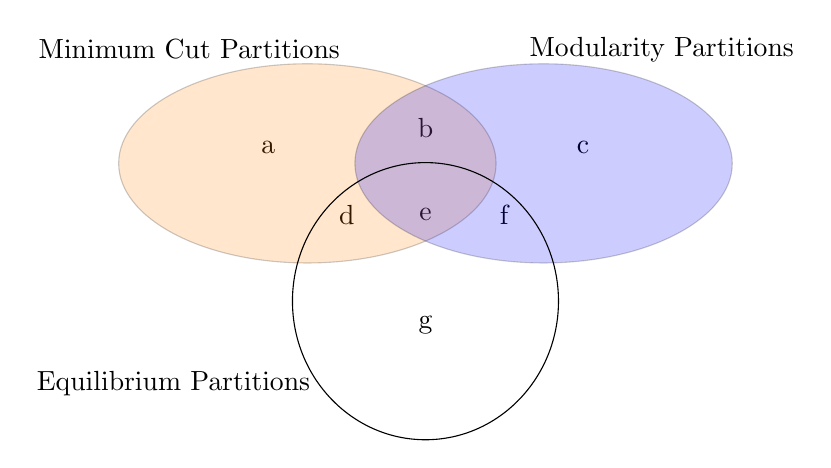
\begin{tikzpicture}
		\node (E1) at (0,0){};
		\node (E2) at (0,1){};
		\node (EQU) at (3,-0.4){};
		\node (Q1) at (6,0){};
		\node (Q2) at (6,1){};
		\node (U1) at (4,-2.5){};
		\node (U2) at (2,-2.5){};
		\node (U3) at (3,-3){};
		
		\node(a) at (1,0.5){a};
		\node(b) at (3,0.75){b};
		\node(c) at (5,0.5){c};
		\node(e) at (3,-0.35){e};
		\node(d) at (2,-0.35){d};
		\node(f) at (4, -0.35){f};
		\node(g) at (3, -1.75){g};
		
		
		\node[fit=(E1)(EQU)(E2), draw, ellipse, fill = orange, opacity = 0.2 ,inner sep=2pt]{};
		\node[fit=(Q1)(EQU)(Q2), draw, ellipse,fill = blue, opacity = 0.2, inner sep=2pt]{};
		\node[fit=(U1)(EQU)(U2), draw, ellipse,inner sep=2pt]{};
		
		\node (Ename) at (0,1.75){Minimum Cut Partitions};
		\node(Qname) at (6,1.75){Modularity Partitions};
		\node(Uname) at (-0.2,-2.5){Equilibrium Partitions};
	\end{tikzpicture}\\
	\vspace{0.5cm}
	\begin{tabular}{ccc}
		
		\textbf{a}&&\textbf{b}\\
		
		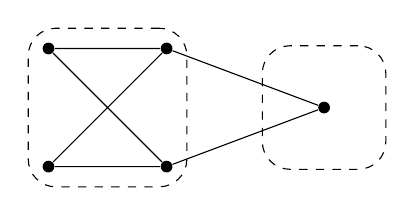
\begin{tikzpicture}
			\node(a) [circle, fill, inner sep =1.5pt] at (0,0){};
			\node(b) [circle, fill, inner sep =1.5pt] at (1.5,0){};
			\node(c) [circle, fill, inner sep =1.5pt] at (0,1.5){};
			\node(d) [circle, fill, inner sep =1.5pt] at (1.5,1.5){};
			\node(e) [circle, fill, inner sep =1.5pt] at (3.5,0.75){};
			
			\draw(b)--(a)--(d)--(c)--(b)--(e)--(d);
			
			\node[fit=(a)(b)(c)(d),dashed,draw, rectangle,rounded corners=10,inner sep=5pt] {};
			\node[fit=(e),dashed, draw, rectangle,rounded corners=10,inner sep=20pt] {};
			
			
			
		\end{tikzpicture}&&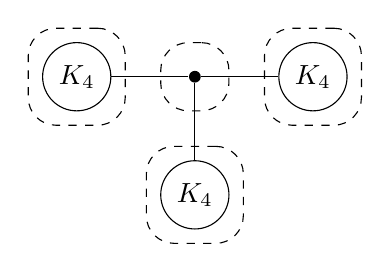
\begin{tikzpicture}
			\node (A) [draw = black, circle] at (0,0){$K_4$};
			\node (B) [draw = black, circle] at (3,0){$K_4$};
			\node (C) [draw = black, circle] at (1.5,-1.5){$K_4$};
			\node(a)[circle, fill, inner sep =1.5pt] at (1.5,0){};
			
			\draw (A)--(a)--(B);
			\draw (a)--(C);
			
			\node[fit=(A),dashed,draw, rectangle,rounded corners=10,inner sep=5pt] {};
			\node[fit=(B),dashed, draw, rectangle,rounded corners=10,inner sep=5pt] {};
			\node[fit=(C),dashed, draw, rectangle,rounded corners=10,inner sep=5pt] {};
			\node[fit=(a),dashed, draw, rectangle,rounded corners=10,inner sep=10pt] {};
			
		\end{tikzpicture}\vspace{0.25cm}\\
		\textbf{c}&&\textbf{d}\vspace{0.25cm}\\
		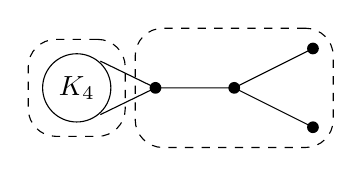
\begin{tikzpicture}
			\node (A) [draw = black, circle] at (1,0){$K_4$};
			\node (B) [circle,fill,inner sep=1.5pt]at (2,0){};
			\node (c) [circle,fill,inner sep=1.5pt]at (3,0){};
			\node (d) [circle,fill,inner sep=1.5pt]at (4,0.5){};
			\node (e) [circle,fill,inner sep=1.5pt]at (4,-0.5){};
			\node[fit=(A),dashed,draw, rectangle,rounded corners=10,inner sep=5pt] {};
			\node[fit=(B)(c)(d)(e),dashed, draw, rectangle,rounded corners=10,inner sep=5pt] {};
			
			\draw (1.3,0.34)--(2,0)--(1.3,-0.34);
			\draw(2,0)--(3,0)--(4,0.5)--(3,0)--(4,-0.5);
		\end{tikzpicture}
		&\hspace{0.5cm} &
		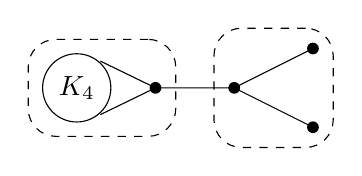
\begin{tikzpicture}
			\node (A) [draw = black, circle] at (1,0){$K_4$};
			\node (B) [circle,fill,inner sep=1.5pt]at (2,0){};
			\node (c) [circle,fill,inner sep=1.5pt]at (3,0){};
			\node (d) [circle,fill,inner sep=1.5pt]at (4,0.5){};
			\node (e) [circle,fill,inner sep=1.5pt]at (4,-0.5){};
			\node[fit=(A)(B),dashed,draw, rectangle,rounded corners=10,inner sep=5pt] {};
			\node[fit=(c)(d)(e),dashed, draw, rectangle,rounded corners=10,inner sep=5pt] {};
			
			\draw (1.3,0.34)--(2,0)--(1.3,-0.34);
			\draw(2,0)--(3,0)--(4,0.5)--(3,0)--(4,-0.5);
		\end{tikzpicture}\vspace{0.5cm}\\
		
		\textbf{e}&&\textbf{f,g}\vspace{0.25cm}\\
		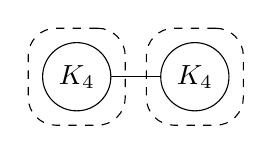
\begin{tikzpicture}
			\node (A) [draw = black, circle] at (0,0){$K_4$};
			\node (B) [draw = black, circle] at (1.5,0){$K_4$};
			
			\draw(A)--(B);
			
			\node[fit=(A),dashed,draw, rectangle,rounded corners=10,inner sep=5pt] {};
			\node[fit=(B),dashed,draw, rectangle,rounded corners=10,inner sep=5pt] {};
		\end{tikzpicture}&& No example yet. \vspace{0.5cm}
		
	\end{tabular}
	\caption{\textbf{Top} A Venn diagram showing Minimum Cut Partitions, Modularity Partitions, and Equilibrium Partitions. \textbf{Bottom} In each of the 6 panels below the Venn diagram is an example (if one is known) of a partition which falls into each region of the Venn diagram. Clusters in the partitions are marked out by dashed lines, For regions f and g, no example has been found, although there is no reason to believe that these regions are empty. }
	\label{Venfig}
\end{figure}
	
	Note that this is a mild strengthening of a result from Brandes et al. \cite{Brandes2006}. We can use these two lemmata to start to get an understanding of partitions which are and are not equilibrium partitions.  	
	
		\begin{corrollary}[Characterization of intersecting partitions]
			Every partition which is a minimum cut partition, but not an equilibrium partition, must have a cluster with a single vertex, $v$. If such a partition is also a modularity partition, $v$ must share an edge with vertices in more than two clusters and no cluster can contain half or more of the neighbors of $v$(Fig. \ref{Venfig}). 
		\end{corrollary}
	
\subsection{Complexity}\label{complexity}

		Almost all partitioning problems are in complexity class $\mathcal{NP}$. Finding a modularity partition, in particular, can be shown to be $\mathcal{NP}$-complete \cite{Brandes2006}. Because of the similarities between these partitions, it's unlikely that we can find an algorithm to solve the BVP that runs deterministically in polynomial time unless the specification of boundary values reduces the problem more than expected, or $\mathcal{NP}$ is in fact $\mathcal{P}$. We can say for certain that finding an equilibrium partition is $\mathcal{NP}$-hard
		
		\begin{theorem} Finding an equilibrium partition is $\mathcal{NP}$-hard.
		\end{theorem}
		\begin{proof}
				To classify the equilibrium partitioning problem into $\mathcal{NP}$ we need only show that there is a condition which is equivalent to being an equilibrium partition and which is checkable in polynomial time\cite{Sipser2006}. To check if a partition is an equilibrium partition one need only determine if every vertex is using a strategy which is an argmax over all strategies of $|\Gamma(v)\cap P^c|$. This requires only $n\cdot |C|\leq n^2$ evaluations.  
		\end{proof}


	\section{Continuous Variations and Applications}\label{continuousvariations}
	\subsection{Sympatric Evolution} \label{sympatricevoluiton}
		In addition to the discrete problem, the continuous variations of this problem are also of some interest, especially in the light of theoretical ecology and the problem of evolution of cooperative behavior.
		%ecology citation
		The discrete problem may do a good job of modeling individual communities and their use of cooperative behaviors, but on larger scales, continuous player spaces and metric strategy spaces may be helpful. 
		
		One question of particular interest is the process of sympatric evolution of cooperative behavior. Sympatric speciation or sympatric evolution is the process of speciation without geographic isolation. Of particular interest is the existence of continuous, \textit{non-constant} strategy profiles across a connected player space. The process of coordination has an intuitive feeling of being centralizing, meaning rare phenotypes are selected against. This tends to put restrictions on what kind of strategic profiles (or phenotypic profiles in the non-game-theoretic case) are possible at equilibrium.  
		\subsection{Mixed Strategy Concept}\label{mixedstrategyconcept}
		Modifying the questions asked in the discrete case may give us tools to understand sympatric evolution of cooperative behavior. The first attempt is to consider a continuous player space with a set of pure strategies $C$ with $|C|=:m$. To have any hope of finding a continuous strategy profile, we consider mixed strategies. This means the strategy space is continuous, but the pure strategies themselves are not comparable. 

			Let $\Omega$ be a domain and $\Delta_m$ be the $m$-simplex in which every mixed strategy lies. Let $\Phi:\Omega \rightarrow\Delta_m$ be a strategy profile. Payoffs are calculated as 
			\begin{equation}\label{mixedstartw}
				w(x|\Phi)=\sum_{i=1}^m \Phi_i(x)\int_\Omega K(x-y)\Phi_i(y)dy =:B(\Phi(x),\Phi(x)) 
			\end{equation} 
			Where $K$ is a familiarity kernel. A familiarity kernel is a distribution describing the frequency of interaction based on relative position. This payoff is a bilinear form which we call $B$. Now the question is: are there any non-constant, continuous $\Phi$ which are Nash Equilibria? 

			This question poses an interesting optimization challenge. It is atypical because we do not seek to optimize a quantity over the entire domain. Instead, we seek to find a $\Phi$ which optimizes a quantity locally for every point in the domain. We are looking for continuous $\Phi$ such that for any $x$,
			\begin{equation}\label{NEcondition}
				w(x|\Phi)\geq w(x|\tilde\Phi)\quad \forall \tilde \Phi(y) = \Phi (y) \text{ for } y\neq x.
			\end{equation}
		
		For the game at hand, with payoff described in \eqref{mixedstartw}. There are no non-constant continuous $\Phi$ which satisfy \eqref{NEcondition}.  
	
		\begin{theorem} {There are no non-constant continuous solutions to \eqref{NEcondition}}
			\end{theorem} 
		\begin{proof} 
			Suppose that $\Phi^\star\in C^0(\Omega;\Delta_m)$ satisfies \eqref{NEcondition} and that it is non-constant. The convolution $K*\Phi^\star_i$ is clearly continuous and  non-constant for any $i$ for which $\Phi^\star_i$ is not constant. Naturally, for any $x\in \Omega$ there is at least one $i$  such that $(K*\Phi^\star_i)(\hat x)\geq (K* \Phi^\star_j)(\hat x)$ for all $j$. 
			
			Moreover, there exists an $\hat x\in \Omega$ such that $(K*\Phi^\star_i)(\hat x)>(K*\Phi^\star_l)(\hat x)>0$ for some $l$. This is because if $(K*\Phi^\star_i)$ was the only non-zero component in all of $\Omega$, then $\Phi^\star$ would be constant and if $(K*\Phi^\star_i)\equiv (K*\Phi^\star_j)$, for all $j$ for which $\Phi^\star_j$ is non-zero, in all of $\Omega$, then again, $\Phi^\star$ would be constant. These two inequalities are attained at the same point somewhere in $\Omega$ because of the continuity of $\Phi^\star$. 
		
			 Thus $\mathbf{a}\cdot (K*\Phi^\star)(\hat x)$ is maximized among all $\mathbf{a}\in \Delta_m$ when $\mathbf{a}=e_i$. Let  \begin{equation}\tilde{\Phi}(x)=\begin{cases} e_i&x=\hat x\\
					\Phi^\star(x)&x\neq \hat x \end{cases}
			\end{equation}
			Because $\{\hat x\}$ is a set of measure zero in $\Omega$, $(K*\tilde{\Phi})\equiv(K*\Phi^\star)$. Thus $w(\hat x, \tilde{\Phi})=(K*\Phi_i^\star)(\hat x)>w(\hat x, \Phi^\star)$, so $\Phi^*$ does not solve \eqref{NEcondition}. This contradiction means that there are no continuous non-constant solutions. 
			
			Additionally, we can say that, for any continuous solution to \eqref{NEcondition}, all the non-zero components of $\Phi$ must be equal in the entire domain. Thus if $\Phi$ has $r\leq m$ strategies expressed, then $\Phi_i=\frac{1}{r}$ for $i=1,...,r$ and $\Phi_i=0$ for $i>r$ (up to relabeling). 
		\end{proof}
	
		This is not altogether surprising. When strategies are discrete and the payoff matrix is the identity, then being around ``nearby" strategies is not beneficial exactly because ``nearby" is meaningless in this context. When strategies do not exist in a metric space, even when we consider mixed strategies, the best response is always to take on the strategy which is most prevalent among those with whom the focal individual interacts. Additionally when strategies do not exist in a metric space, the model is not entirely biologically relevant. Cooperative behaviors are complex and can frequently be compared to one another. Those most complicated cooperative behaviors like languages and social norms have a notion of mutual intelligibility where, even if the two strategies are not identical, they are close enough to give some fitness benefit. 
		\subsection{Comparable Strategy Concept}\label{comparablestrategyconcept}	
		Therefore, instead of only considering the identity payoff matrix, we ought to look at strategies which are comparable under a ``blurred" payoff matrix. Consider this symmetric payoff matrix
		\begin{equation}\label{BlurredPayoffMatrix}
			\begin{bmatrix}
				1&\alpha&0\\
				\alpha&1&\alpha\\
				0&\alpha&1
			\end{bmatrix}
		\end{equation}
		
		Under this new blurred payoff matrix, we have a degree of similarity between strategies. Strategy 2 is mutually intelligible with strategies 1 and 3, symmetrically, but strategies 1 and 3 are not mutually intelligible. This results in some strategy profiles which are Nash equilibria under the new payoff matrix but were not Nash equilibria under the identity payoff matrix (Fig. \ref{BlurredNE}).   
	
		\begin{figure} [h!]
			\centering
			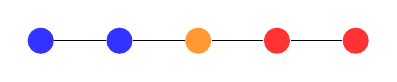
\begin{tikzpicture}
				\node (A) at (0,0)[fill = blue, circle, opacity = 0.8]{};
				\node (B) at (1,0)[fill = blue, circle, opacity = 0.8]{};
				\node (C) at (2,0)[fill = orange, circle, opacity = 0.8]{};
				\node (D) at (3,0)[fill = red, circle, opacity =0.8]{};
				\node (E) at (4,0)[fill = red, circle, opacity = 0.8]{};
				
				\draw (A)--(B)--(C)--(D)--(E);
			\end{tikzpicture}
			\caption{A strategy profile which is a Nash equilibrium for the game with payoff matrix \eqref{BlurredPayoffMatrix} if and only if $\alpha\geq \frac{1}{2}$.}
			\label{BlurredNE}
		\end{figure}
		This simple example poses some interesting questions. In a more general setting, are there ``recognition thresholds" which define critical regions where sympatric evolution of cooperative behavior can occur? Are there critical domain sizes? To translate this to the continuous case where it is more analytically tractable, we can imagine the familiarity kernel taking the place of the graph structure from the discrete case. To represent a ``blurred" payoff matrix, we may equip our strategy space with a metric, $d$, and use a recognition function, $\rho$, which determines how much of the fitness benefit an individual gets as a function of the distance between two strategies.   
	
		Consider the game played in the domain $\Omega$. Instead of using linear combinations of pure incomparable strategies, think of a strategy profile $\Phi:\Omega \rightarrow M$ which gives the payoff
		\begin{equation}
			w(x|\Phi)= \int_\Omega K(x-y)\rho(d(\Phi(y),\Phi(x)))dy.
		\end{equation}
		Here $M$ is a metric space with the metric $d$, $\rho(y)$ is a recognition function which has $\rho (0)=1$ and $\rho(r)=0$ for $r>r^*$, which we call the critical recognition distance. Under these conditions, we can indeed find continuous non-constant strategy profiles which are Nash equilibria.  
	
		\begin{example}
			Let $\Omega$ be a domain in $\mathbb{R}^n$, let $\rho(r)=1$ for $r\leq r^*$ and $0$ otherwise, and let $K(x)=\frac{1}{\alpha(n)\kappa^n}$ for $|x|<\kappa$ and $0$ otherwise where $\alpha(n)$ is the volume of the unit ball in $n$ dimensions. Let the strategy space $M$ be a subset of $\mathbb{R^m}$ so the metric is simply $|\cdot|$.
			\begin{equation}
				w(x|\Phi)=\int_\Omega K(x-y)\rho(|\Phi(y)-\Phi(x)|)dy
			\end{equation} 
			Under these conditions, any $\Phi \in C^{0,1}(\Omega; M)$ with Lipschitz constant less than $\frac{r^*}{\kappa}$ is a Nash equilibrium.
		\end{example}
		
		\begin{proof}
			Observe that the maximum fitness for any $x\in \Omega$ is \begin{equation}
				w(x|\Phi)=\int_\Omega K(x-y)dy=\frac{1}{\alpha(n)\kappa^n}|\Omega\cap supp_y(K(x-y))|
			\end{equation}
			where $supp_y(K(x-y))$ means those $y$ values which make $K(x-y)>0$. 
			Clearly, if a strategy attains this fitness maximum for all $x\in \Omega$, it is a Nash equilibrium. Let $\Phi\in C^{0,1}(\Omega;M)$ with Lipschitz constant $<\frac{r^*}{\kappa}$ Thus, for any $x,y\in \Omega$, $|\Phi(x)-\Phi(y)|\leq \frac{r^*}{\kappa}|x-y|$.
			
			Select any $x\in\Omega$ and consider $w(x|\Phi)$. 
			\begin{equation}
				\begin{split}
					w(x|\Phi)&=\int_\Omega K(x-y)\rho(|\Phi(x)-\Phi(y)|)dy\\
					&=\frac{1}{\alpha(n)\kappa^n}\int_{\Omega\cap supp_y (K(x-y))}\rho(|\Phi(x)-\Phi(y)|)dy
				\end{split}
			\end{equation} 
			By the assumption that $\Phi$ has a Lipschitz constant less than $\frac{r^\star}{\kappa}$, we know that in $\Omega\cap supp_yK(x-y)$ we have $|\Phi(x)-\Phi(y)|< \frac{r^*}{\kappa}|x-y|\leq r^*$. Therefore $\rho(|\Phi(x)-\Phi(y)|)=1$ in this region and we have the fitness
			\begin{equation}
				w(x|\Phi)=\frac{1}{\alpha(n)\kappa^n}|\Omega\cap supp_y(K(x-y))|
			\end{equation}
			Because this is the maximum achievable fitness for all $x\in \Omega$, it is a Nash equilibrium trivially. 
		\end{proof} 
		
	
		In this example, we can see that if $r^*\rightarrow0$, then a continuous non-constant Nash Equilibrium is impossible. We can prove this easily when $\Omega$ is closed and bounded and when $M\subset \mathbb{R}$ by considering the maxima of $\Phi$. With fewer restrictions on the domain and range of $\Phi$ we may still be able to argue the same thing. This is not surprising as it returns us to the case where the payoff matrix is the identity matrix and there is no mutual intelligibility.  
		
		Additionally, if $\Omega$ is bounded and $\kappa> diam(\Omega)$, we again see that there could be no non-constant continuous Nash equilibria unless $r^\star>diam(\Phi(\Omega))$.  
		
		This second limiting example has a satisfying and natural analogue in the discrete case. If we imagine the familiarity kernel to be related to the structure of the graph as before, the graph corresponding to the the kernel with large $\kappa$ is the complete graph, as every player interacts with every other player. In theorem \ref{KnTheorem} we proved that no non-constant Nash equilibria can exist in such a graph.
	
		In a more general setting, it is interesting to observe the relationship between the familiarity kernel and the recognition function as it is relates to the admittance of non-constant continuous Nash equilibria. In the future, it is our goal to prove more general results about when these examples of sympatric evolution of cooperative behaviors can occur with more reasonable familiarity kernels and recognition functions. 
	\section*{Conclusion}\label{conclusion} 
	Each of these proposed investigations offer a unique way of thinking about coordination behavior in space. In section \ref{equilibria and stability} we consider the discrete space case through time. Where, previously, economists have investigated this question for simple graphs with nice symmetric reductions, we seek to find more general results about equilibria and stability of this system through energy like estimates and extremal graph theoretic techniques. In section \ref{boundaryvalueproblem}, we consider the same discrete space, but instead of the time evolution, we think of it as a BVP. Borrowing from graph partitioning, we seek to find a way to give an equilibrium interpolation given a set of boundary values. Lastly, in section \ref{continuousvariations}, we consider a similar problem continuously in space and investigate the ways that qualities of familiarity and recognition change the kinds of strategic profiles that can exist at equilibrium. Each of these investigations provide us with exciting ways to think about coordination in space. Whether it be in economics or behavioral ecology, this game can help us understand how coordinated behavior arises and what patterns of coordination we can expect at equilibrium.  
	\bibliographystyle{plain}
	\bibliography{structuredcoord.bib}
\end{document}


          
